\documentclass{article}
\usepackage{tikz}

\begin{document}

\begin{figure}[h]
    \centering
    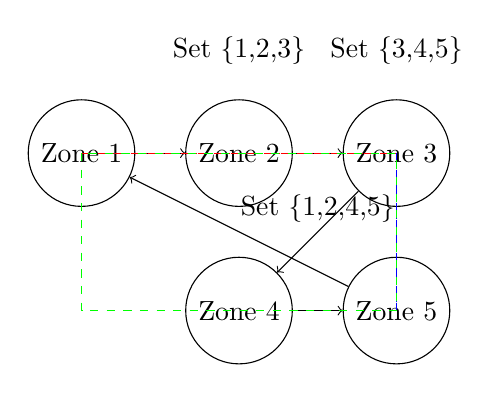
\begin{tikzpicture}
        % Define the nodes (zones)
        \node[circle, draw] (Zone1) at (0,0) {Zone 1};
        \node[circle, draw] (Zone2) at (2,0) {Zone 2};
        \node[circle, draw] (Zone3) at (4,0) {Zone 3};
        \node[circle, draw] (Zone4) at (2,-2) {Zone 4};
        \node[circle, draw] (Zone5) at (4,-2) {Zone 5};

        % Draw the connections between zones
        \draw[->] (Zone1) -- (Zone2);
        \draw[->] (Zone2) -- (Zone3);
        \draw[->] (Zone3) -- (Zone4);
        \draw[->] (Zone4) -- (Zone5);
        \draw[->] (Zone5) -- (Zone1);

        % Highlight the sets where White can pass back components
        \draw[dashed, red] (Zone1) rectangle (Zone3);
        \draw[dashed, blue] (Zone3) rectangle (Zone5);
        \draw[dashed, green] (Zone1) rectangle (Zone5);

        % Add labels to indicate the sets
        \node[above=0.5cm] at (2,0.5) {Set \{1,2,3\}};
        \node[above=0.5cm] at (4,0.5) {Set \{3,4,5\}};
        \node[above=0.5cm] at (3,-1.5) {Set \{1,2,4,5\}};

    \end{tikzpicture}
    \caption{Diagram representing the zones and the sets where White can pass back components.}
    \label{fig:zones}
\end{figure}

\end{document}